% !Mode:: "TeX:UTF-8"
%!TEX program  = xelatex

% =============================================================================
% 这里只是一个自用模板的分享。
% 本模板基于国赛论文模板修改,若侵即删,联系邮箱:alordzero@hotmail.com。
% 没有系统学过LaTeX,存在一些小的问题没好好弄。
% 像是每个二级三级标题与上面正文之间的行距我是凭感觉调的,非精确到数值。
% 不需要的部分注释掉就好了。
% latex的表格、图、算法等浮动体的顺序比较讲究,需要自己摸索。
% 文本内容纯粹是整活,别认真。
% 
% LaTeX分为导言区和正文区:
% 1. 导言区规范格式,正文区编辑内容。
% 2. 导言区一般要导入各种宏包,类似python里导入库,对应\usepackage命令。
% 3. 一些自定义的格式,也在导言区完成,类似于python里自定义函数,对应\newcommand和\renewcommand命令。
% 4. 正文区以\begin{document}{开始,以\end{document}结尾。
% =============================================================================

% 这里要导入MCM数模国赛论文模板中的cumcmthesis,里面定义了很多基础的东西
\documentclass{cumcmthesis}
% 改了cumcmthesis里的一些东西,要符合毕设格式的标准
% 1. 给一级标题、二级标题的黑体加粗。
% 2. 页边距改成了毕设的标准 top=30mm,bottom=25mm,left=30mm,right=20mm。

% 导入必要的宏包,国赛模板里本身就有导入的部分
\usepackage{multicol}
\usepackage{url}
\usepackage{cases}
\usepackage{array}
\usepackage{booktabs}
\usepackage{geometry}
\usepackage{fancyhdr}
\usepackage{mathdots}

% 下面是宏包补充

% 1. 参考文献目录按照 GBT7714 标准
\usepackage{gbt7714}
% 本模板强烈建议使用bibtex编排参考文献,参考文献顺序按照正文中引用顺序自动编排
% bibtex GBT7714格式参考文献提供者(侵删):https://github.com/zepinglee/gbt7714-bibtex-style
% bibitem方法只能手动排参考文献的顺序,不建议使用

% 2. 启用交叉引用超链接跳转
\usepackage{hyperref}
\hypersetup{colorlinks = true,linkcolor = black, anchorcolor = black, citecolor = black, urlcolor = black, pdfauthor = author}

% 3. 缩短参考文献展示间距
\usepackage{bibspacing}
\setlength{\bibspacing}{0\baselineskip}
% 用到了bibspacing.sty文件
% 方法参考来源:https://blog.csdn.net/weixin_40520963/article/details/105137544

% 4. 基于algorithm2e的中文算法浮动体(无行号)
\usepackage[ruled,lined,boxed,commentsnumbered]{algorithm2e}[1]
\renewcommand{\algorithmcfname}{算法 -} %定义算法的名字,自动接上编号,类似caption
% \renewcommand{\algorithmcfname}{算法4 -} %假如是在第4章,加个4,就显示为算法4-1
\SetKwInput{KwIn}{输入}
\SetKwInput{KwOut}{输出}

% 5. 显著性*上标,需要用到这个
\usepackage{threeparttable}

% 6. 用于强制给表格某一元素居中
\usepackage{makecell}

% 7. 附录代码MATLAB宏包
\usepackage{listings,matlab-prettifier} % MATLAB 美化包
\lstset{style=Matlab-editor,numbers=left,frame=single}

% 8. 如果表格内容过长需要自动换行,要用到tabularx宏包
\usepackage{tabularx}
\usepackage{ragged2e}
\renewcommand\tabularxcolumn[1]{m{#1}} % 垂直居中 for vertical centering text in X column

% 下面是一些自定义的格式修改和前置准备

% 1. 公式纯数字编号改为按章节编号
\numberwithin{figure}{section}
\numberwithin{table}{section}
\numberwithin{equation}{section}

% 2. 文献交叉引用改为处于上标
\makeatletter
\def\@cite#1#2{\textsuperscript{[{#1\if@tempswa , #2\fi}]}}
\makeatother

% 3. 定义英文摘要环境
\newcommand{\enabstractname}{Abstract}
\newenvironment{enabstract}{
	\par\large
	\noindent\mbox{}\hfill{\bfseries\zihao{3}\enabstractname}\hfill\mbox{}\par
	\vskip 2.5ex}{\par\vskip 2.5ex}

% 4. 封面格式的前置(忘了参考来源是哪)
\makeatletter
\newcommand\dlmu[2][4cm]{\hskip1pt\underline{\hb@xt@ #1{\hss#2\hss}}\hskip3pt}
\makeatother

% 5. 做书脊的前置准备
\usepackage{tikz} % 用于书脊的灰色长方形的宏包
\renewcommand{\title}[1]{\def\spinetitle{#1}}
\renewcommand{\author}[1]{\def\spineauthor{#1}}
\newcommand{\institute}[1]{\def\spineinst{#1}}
\newcommand{\makespine}{
	\linespread{1.0}  % 书脊部分需要临时改为一倍行距
	\vspace*{28mm} % 调整书脊字的间距用的(如果标题过长或过短,需要调这里的间距)
	\spinetitle
	\vfill % 调整书脊字的间距用的
	\spineauthor
	\vfill % 调整书脊字的间距用的
	\spineinst
	\vfill % 调整书脊字的间距用的
} % 修改自国科大标准书脊,参考来源:https://github.com/mohuangrui/latexspine


% =============================== 分割线 ======================================
% 开始正文区
\begin{document}{
		
% 1.5倍行距,该命令只影响后面的内容
\linespread{1.5}
\pagestyle{empty} % 正文之前都不编页码	


% =============================================================================
% 封面页
% =============================================================================
% 广工logo(一个文字,一个校徽)
\begin{figure}[h]
	\nonumber % 该图不编号
	\centering % 居中
	\vspace{-0.2em} % 调整垂直间距(纯手调,下同)
	\hspace*{-31em} % 调整水平间距(纯手调,下同)
	
\includegraphics[width=2.09cm]{figures/校徽logo.jpg}
\end{figure}

\begin{figure}[h]
	\nonumber
	\centering
	\vspace{-1.8em}
	\hspace*{0em}
	
\includegraphics[width=10.59cm]{figures/文字logo.jpg}
	\vspace{-1.8em}
\end{figure}

% 论文类型
\begin{center}
	\zihao{1} % 一号黑体加粗
	\hspace*{1em}
	\vspace{0em}
	\textbf{\boldheiti 本科毕业设计(论文)} % \bfseries\boldheiti 或者 \textbf{\boldheiti ***} 才可以实现黑体加粗
	\vspace{0.7em}
\end{center}

% 论文标题(这里就可以写上自己的标题了,撑个两行还是可以的)
\begin{center}
	\zihao{2} % 二号黑体加粗
	\vspace{0.5em}
	\textbf{\boldheiti 基于生成型预训练变换模型的降重猪怪谈研究}
\end{center}

% 个人信息(写上自己的个人信息)
\begin{center}
	\vspace{2em}
	\zihao{3} % 三号黑体加粗
	\begin{tabular}{rl}
	&\\
	&\makebox[4em][s]{\textbf{\boldheiti 学院}}\hspace{0.2cm}\dlmu[6cm]{\textbf{\boldheiti 五金学院}}\\
	&\makebox[4em][s]{\textbf{\boldheiti 专业}}\hspace{0.2cm}\dlmu[6cm]{\textbf{\boldheiti 五金工程}}\\
	&\makebox[4em][s]{\textbf{\boldheiti 年级班别}}\hspace{0.2cm}\dlmu[6cm]{\textbf{\boldheiti xxxx级y班}}\\
	&\makebox[4em][s]{\textbf{\boldheiti 学号}}\hspace{0.2cm}\dlmu[6cm]{\textbf{\boldheiti 114514}}\\
	&\makebox[4em][s]{\textbf{\boldheiti 学生姓名}}\hspace{0.2cm}\dlmu[6cm]{\textbf{\boldheiti 永强}}\\
	&\makebox[4em][s]{\textbf{\boldheiti 指导教师}}\hspace{0.2cm}\dlmu[6cm]{\textbf{\boldheiti 丧彪}}\\
	&\\
	\end{tabular}
\end{center}

% 底下日期
\begin{center}
	\vspace{0em}
	\zihao{3} % 三号黑体加粗
	\textbf{\boldheiti xxxx年5月}
\end{center}

% 封面背面白纸(暂时用不到可以注释掉)
\newpage
\mbox{} % 空白页必须填一个空内容\mbox{},不然\newpage起不到作用

% =============================================================================
% 书脊页
% =============================================================================
\newpage

% 书脊灰色长方形条
\begin{tikzpicture}[remember picture,overlay]
	\fill[gray!50] ([shift={(1.1cm,16cm)}]current page.center) rectangle ++(-1.2cm,-\paperheight-5cm);
\end{tikzpicture}

% 填上自己的信息,\par后必须留空格
\begin{center}
	% 论文中文题目(如果标题过长或过短,需要回到导言区调\vspace*的间距)
	\title{\bfseries\boldheiti\zihao{4}基\par 于\par 生\par 成\par 型\par 预\par 训\par 练\par 变\par 换\par 模\par 型\par 的\par 降\par 重\par 猪\par 怪\par 谈\par 研\par 究\par}
	% 论文作者(四号黑体加粗)
	\author{\bfseries\boldheiti\zihao{4}永\par 强}
	% 学校名称(小四号黑体加粗)
	\institute{\bfseries\boldheiti\zihao{-4}五\par 金\par 学\par 院\par}
	\makespine % 生成书脊
	\linespread{1.5} % 调回1.5倍行距
\end{center}

% 书脊背面白纸(暂时用不到可以注释掉)
\newpage
\mbox{}

% =============================================================================
% 中文摘要页
% =============================================================================
\newpage

% 摘要正文(小四号宋体,宋体/times new roman是正文默认字体)
% 无内容的空行有换行的含义,无空行的内容都是接在一起的
\zihao{-4} % 加个负号就是小四号
\begin{abstract}

在学术圈子里,有一种名为“降重猪”的神秘生物的传说。据说,这种生物能够降低论文的查重率,让那些信仰它的人轻松通过学术考验。这种传说可能源于一些学生或者学者在面对写作压力和查重难题时的心理寄托,也可能是一种网络文化现象的反映。然而,这种传说的真实性和合理性一直没有得到科学的验证,也没有被正式的学术机构或者期刊所承认或者接受。相反,这种传说可能会误导一些不懂得如何正确写作和引用的人,导致他们忽视论文的质量和原创性,甚至触犯学术道德和规范。

本文旨在探讨“降重猪”传说的起源、流传和影响,以及它对学术道德和创新的潜在危害。本文采用了文献综述、网络分析和问卷调查等方法,从历史、社会、心理和教育等角度进行了多维度的分析。本文首先回顾了“降重猪”传说的出现背景和发展过程,然后通过对网络平台上关于“降重猪”的内容和评论的抓取和分析,揭示了这种传说在不同群体和领域中的流行程度和态度差异,以及它所反映出的网络文化特征和价值观倾向。接着,本文通过设计和发放在线问卷,收集了不同年龄、性别、学历、专业和职业等背景的人对于“降重猪”传说的认知、态度和行为的数据,并进行了统计分析和比较,探讨了这种传说对于人们的学习动机、写作习惯、创新能力和道德观念等方面的影响。

本文的实证分析结果表明,“降重猪”传说是一种具有较强社会影响力和文化意义的网络现象,它既反映了一些人在面对学术压力时的无奈和求助,也暴露了一些人在写作过程中缺乏规范意识和创新精神。本文发现,“降重猪”传说在不同群体中有不同的流行程度和接受度,其中以年轻人、学生、非专业人士等为主要受众。本文还发现,“降重猪”传说对于人们的学习动机、写作习惯、创新能力和道德观念等方面有不同程度的负面影响,尤其是对于那些缺乏自信、自律和自主性的人。本文认为,“降重猪”传说不仅是一个有趣的怪谈,更是一个值得关注和警惕的社会问题,它需要我们从多个层面进行干预和改善,提高人们的学术素养和创新意识。

本文使用\LaTeX 进行排版。\\ % 双斜杠必须要紧挨着最后一段文本

% “关键词”三个字是四号黑体
\par\noindent\zihao{4}\textbf{\boldheiti 关键词:}
\zihao{-4} 降重猪\quad 网络现象\quad 统计分析\quad 关键词4\quad 关键词5

\end{abstract}      

% 中文摘要背面白纸
\newpage
\mbox{}

% =============================================================================
% 英文摘要页
% =============================================================================
%\newpage

% 摘要正文
\begin{enabstract}
	
In academic circles, there is a legend of a mysterious creature called the plagiarism-reducing pig. It is said that this creature can reduce the plagiarism rate of papers, and let those who believe in it easily pass the academic test. 

This article is typeset using \LaTeX.\\
\par\noindent\zihao{4}\textbf{Key words:}
\zihao{-4} Plagiarism-reducing Pig, Network Phenomenon, Statistic Analysis, Keyword 4, Keyword 5

\end{enabstract}

% 英文摘要背面白纸(如无需要可以注释掉)
\newpage
\mbox{}

% =============================================================================
% 目录页
% =============================================================================
\newpage
\pagestyle{empty} % 保证目录页没有不编页码
\tableofcontents % 放置目录

% 目录背面白纸(这里目录较短,一般两页目录就注释掉,打印才不会出错)
%\newpage
%\mbox{}

% =============================================================================
% 第一章开始
% =============================================================================
\newpage

% 恢复可以编页码
\pagestyle{fancy}
\fancyhf{}
\pagestyle{plain}
\setcounter{page}{1} % 设置本页页码,只用设置一次,后续页会自动生成

% 一级标题,可以自定义修改(编号会自动生成)
\section{绪论}
% 二级标题,可以自定义修改(编号会自动生成)
\subsection{研究背景及意义}
% 三级标题,可以自定义修改(编号会自动生成)
\subsubsection{研究背景}

据说在古老的传说中,有一种名为“降重猪”的神秘生物。传说中,这种生物能够降低论文的查重率,让那些信仰它的人轻松通过学术考验。
据说,当你需要写一篇论文并且担心自己的作品会被查重系统识别出抄袭时,你可以拜这种降重猪,希望它能降低你论文的相似度得分。一些人称,这种生物可以通过神秘的方式影响检测系统,使得它们无法完全识别文本的原创性。
当然,也有一些人对这种传说持怀疑态度,并认为降重猪只是一个虚构的故事。但无论如何,这个有趣的传说已经在学术圈子里流传很久了,成为了一个独特的怪谈。

\vspace{-0.6em} % 默认与上节文本的距离有点大,目测减了0.6em的距离比较舒服
\subsubsection{研究意义}

\textcolor[RGB]{0,0,255}{比如我这个地方还没改好,我怕忘记了,就标成蓝色。}

\vspace{-0.6em} % 默认与上节文本的距离有点大,目测减了0.6em的距离比较舒服
\subsubsection{研究方法}

本研究采用文献分析法和实证分析法来探究降重猪的现象。

\noindent(1)文献分析法 % \noindent表示取消缩进

通过文献分析法

\noindent(2)实证分析法

% 百分号必须写成$\%$,%是latex的注释符号
通过实证分析法,降重率为80$\%$。


\vspace{-0.6em} % 默认与上节文本的距离有点大,目测减了0.6em的距离比较舒服
\subsubsection{论文结构与技术路线}

本文一共分为3个部分,具体安排如下:

论文第1章是绪论环节,\textcolor[RGB]{0,0,255}{包括...}

论文第2章是文献综述,\textcolor[RGB]{0,0,255}{包括...}

论文的最后环节是结论。


% =============================================================================
% 第二章开始
% =============================================================================

\newpage
\section{文献综述}

\textcolor[RGB]{0,0,255}{本章的引言部分,我怕忘记了,就标成蓝色。}

\vspace{-0.6em}
\subsection{学术文化现象}

降重猪是一种神秘的学术文化现象,它指的是一种能够降低论文的查重率,让那些信仰它的人轻松通过学术考验的神秘生物。关于降重猪的传说,已经在学术圈子里流传很久了,成为了一个独特的怪谈。本文旨在对降重猪的现象进行一个初步的文献综述,从以下三个方面来梳理和分析相关的资料:一是降重猪的起源和传播;二是降重猪的功能和效果;三是降重猪的评价和争议。

\vspace{-0.6em}
\subsection{文献评述}

综上所述,降重猪是一个值得关注和研究的学术文化现象,它涉及到多个方面的问题和挑战,如学术抄袭、学术伦理、学术创新、网络文化等。本文通过对相关文献资料的梳理和分析,对降重猪的现象进行了一个初步的文献综述,从降重猪的起源和传播、功能和效果、评价和争议三个方面来展开讨论。本文旨在为后续的深入研究提供一些基础和参考,也希望能够引起更多人对降重猪这一有趣而又神秘的现象的关注和思考。


% =============================================================================
% 第三章开始
% =============================================================================

\newpage
\section{实证分析}

\textcolor[RGB]{0,0,255}{本章的引言部分,我怕忘记了,就标成蓝色。}

\vspace{-0.6em}
\subsection{模型介绍}

\subsubsection{期权定价方法}

不整活了(doge),复杂的tex公式语法需自学,下面用一些写过的推导做演示:

例子1:经典的用Black-Scholes-Merton(BSM)模型其形式如公式\eqref{布朗运动}所示。% 用\eqref对公式进行交叉引用

\begin{equation}
	\label{布朗运动} % 该公式的标签
	\setlength\abovedisplayshortskip{-0.3cm} % 调整公式与上下文的间距
	\setlength\belowdisplayshortskip{0.5cm} % 调整公式与上下文的间距
		\begin{cases} % 带花括号的多行公式
		\text{d}S_t=\mu S_t dt+\sigma S_t \text{d}W_t\\ % 用斜杠换行
		\text{d}W_t=\epsilon\cdot \sqrt{ \text{d}t},\epsilon \sim N(0,1)
		\end{cases}
\end{equation}

$\text{d}W_t$表示维纳过程(Wiener Process),$\mu$被称作漂移项(drift),$\sigma$被称作扩散项(volatility),因此也符合伊藤过程(Ito Process),可以使用伊藤引理(Ito Lemma)来辅助求解随机微分方程

例子2:VAR模型\cite{sims1980}的移动平均形式表示如下:% 用\cite对文献进行交叉引用,文献简称sims1980是在ref.bib文件里定义的。多个文献同时引用,用逗号隔开。

\begin{equation}
	\label{VAR(p)模型移动平均形式}
	\setlength\abovedisplayshortskip{-0.3cm}
	\setlength\belowdisplayshortskip{0.5cm}
		{y}_t={\phi}+\sum^\infty_{h=0}{B}_h{u}_{t-h}
\end{equation}

系数矩阵$B$满足如下递归关系,这里放一个脚注\protect\footnotemark[1]: % 引用脚注

\begin{equation}
	\nonumber % 不给这个公式编号
	\setlength\abovedisplayshortskip{-0.3cm}
	\setlength\belowdisplayshortskip{0.5cm}
		\begin{aligned} % 无括号的多行公式
		{B}_0 &= {I} \\
		{B}_1 &= {A}_1{B}_0 \\
		{B}_2 &= {A}_1{B}_1 + {A}_2{B}_0 \\[-5pt] % [-5pt]用来调整间距
		\vdots\\[-10pt] % [-5pt]用来调整间距
		\end{aligned}
\end{equation}

% 编辑脚注内容
\footnotetext[1]{\zihao{6}脚注内容,字号为6号字体}

表格就很讲技术了,普通表格浮动体展示(三线表,内部可以放TeX公式):

\begin{table}[htbp]
	\setlength{\abovecaptionskip}{0.1cm}
	\setlength{\belowcaptionskip}{-0.1cm}
	\centering % 表格整体是居中的
	\zihao{5} % 表格内容字体大小为五号
	\caption{表格名字}
		\begin{tabular*}{\hsize}{@{\extracolsep{\fill}}cccccc}
			\toprule % 顶端粗线
				& $y_1$ & $y_2$ & $\cdots$ & $y_{N}$\\[2pt] % [2pt]用来加2pt间距
			\hline % 中间细线
			$\qquad y_1$ & 111 & 222 & 333 & 444\\[2pt] % 如果觉得内容太靠边了,可以用$\quad$调整一下
			$\qquad y_2$ & $\sum^N_{i=1,i\neq 1}\widetilde{\theta}^H_{i\leftarrow 1}$ & $\sum^N_{i=1,i\neq 2}\widetilde{\theta}^H_{i\leftarrow 2}$ & $\cdots$ & $\sum^N_{i=1,i\neq N}\widetilde{\theta}^H_{i\leftarrow N}$\\[2pt]
			\bottomrule % 底端粗线
		\end{tabular*}
	\label{溢出表}
\end{table}

\newpage % 有时候希望文字进入到下一页,就在文本前另起新一页

自动换行表格浮动体展示(这种表格行距比较窄):

\begin{table}[htbp]
	\setlength{\abovecaptionskip}{0.1cm}
	\setlength{\belowcaptionskip}{-0.1cm}
	\centering
	\zihao{5}
	\caption{自动换行表格}
	\begin{threeparttable}
		\begin{tabularx}{\textwidth}{c|X}
			\toprule
			\multicolumn{1}{c|}{汇率制度} & \multicolumn{1}{c}{国家}\\
			\hline
			自由浮动汇率&国家1、国家2、国家3、国家4、国家5、国家6、国家7、国家8、国家9、国家10、国家11、国家12\tnote{*}\\
			\hline
			有管理的浮动汇率&国家13、国家14、国家15、国家16\\
			\bottomrule
		\end{tabularx}
		
		\begin{tablenotes}
			%\centering
			\zihao{-5}
			\item 注:表格注释内容,例如*表示5$\%$上显著。
		\end{tablenotes}
	\end{threeparttable}
	
	\label{}
\end{table}

复杂表格浮动体演示:

\begin{table}[h]
	\setlength{\abovecaptionskip}{0.1cm}
	\setlength{\belowcaptionskip}{-0.1cm}
	\centering
	\zihao{5}
	\caption{复杂表格浮动体}
	
	\begin{tabular*}{\hsize}{@{\extracolsep{\fill}}ccccc}
		\toprule
		\multirow{2}*[-0.6ex]{$\quad $行}&\multicolumn{2}{c}{总列名1}&\multicolumn{2}{c}{总列名2}\\[-2pt] % 合并单元格
		\cmidrule(lr){2-3}\cmidrule(lr){4-5} % 只在2到3列,4到5列加条横线
		&字列名1&字列名2&字列名1&字列名2\\[-2pt]
		\midrule
		\multirow{2}*{$\quad$ 行名1}&111&222&333&444\\[-2pt] % 如果觉得内容太靠边了,可以用$\quad$调整一下
		~ & \multicolumn{2}{c}{333} & \multicolumn{2}{c}{777}\\[-2pt]
		\hline
		\multirow{2}*{$\quad$ 行名2}&111&222&333&444\\[-2pt]
		~ & \multicolumn{2}{c}{333} & \multicolumn{2}{c}{777}\\[-2pt]
		\bottomrule
	\end{tabular*}
	
	\begin{tablenotes}
		%\centering % 要居中的话就取消注释这行
		\zihao{-5}
		\item 注:内容内容内容十五字十五字十五字。
	\end{tablenotes}
	
	\label{}
\end{table}

图片浮动体展示(支持位图和矢量图):

\begin{figure}[htbp]
	\setlength{\abovecaptionskip}{0.2cm} % 调整前后间距
	\setlength{\belowcaptionskip}{-0.2cm} % 调整前后间距
	\centering
	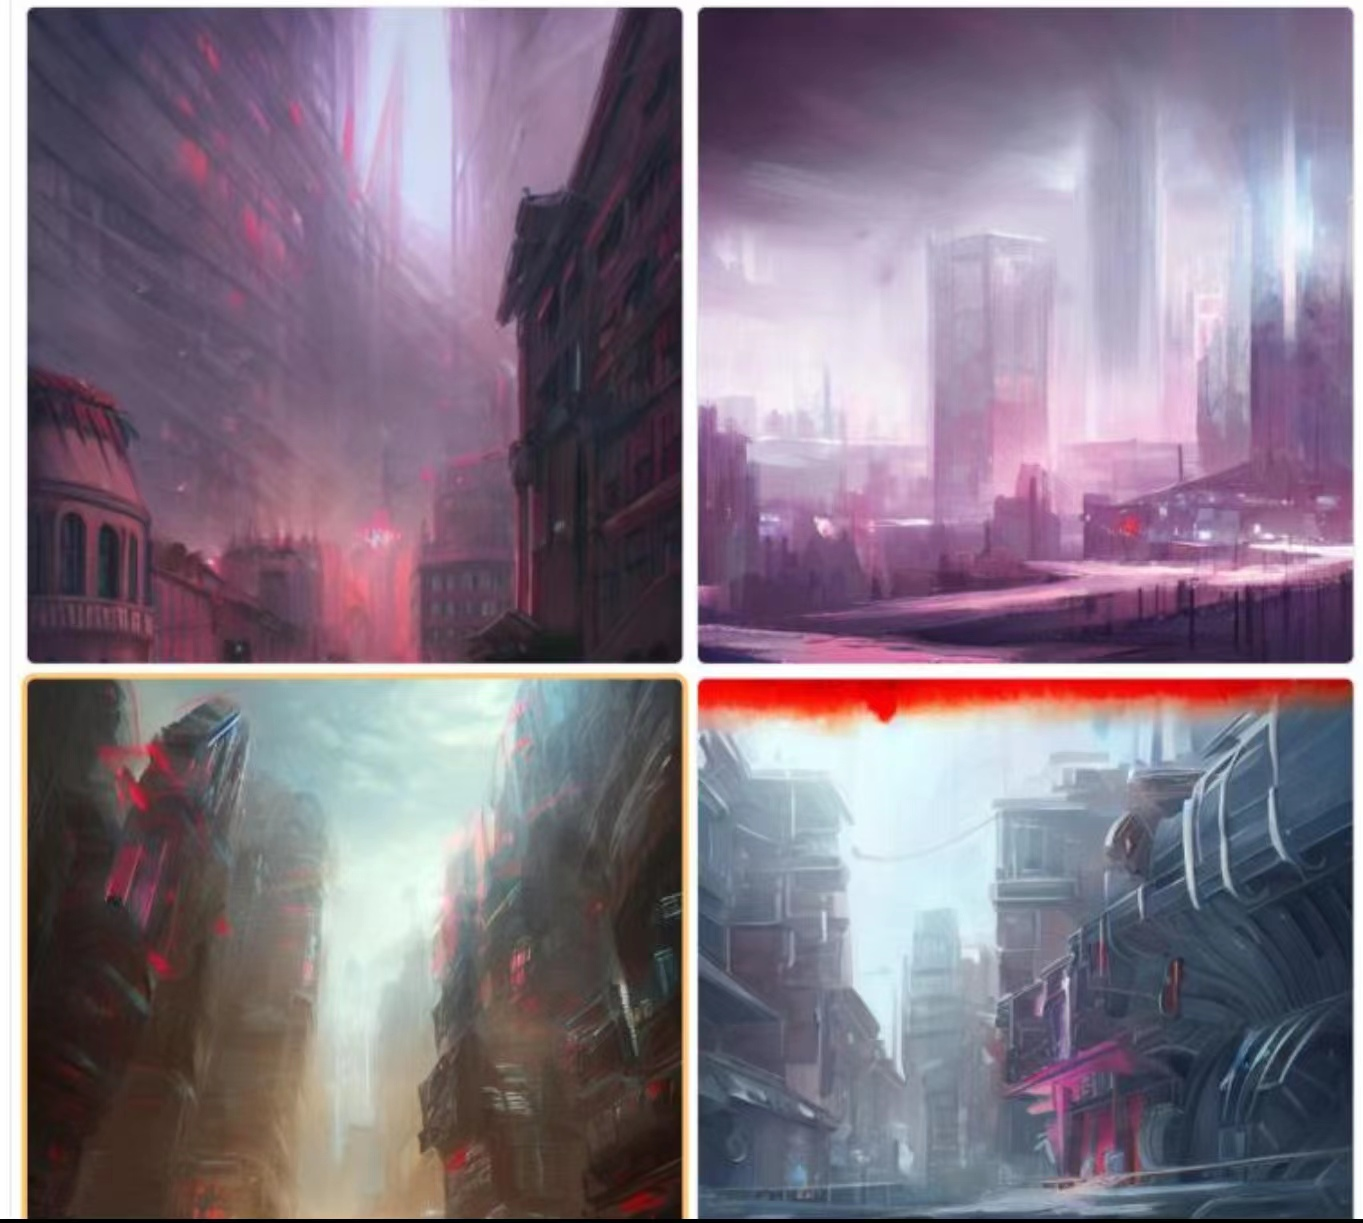
\includegraphics[width=10cm]{figures/AI生成图片.jpg} % 图片路径,默认在figure文件夹里,图片宽度可以写6cm这样的具体数字的宽度,也可以写成\textwidth表示撑满文段的宽度。支持jpg./.png等位图格式,也可以用.pdf/.eps等矢量图。
	\caption{AI生成图片}
	\label{}
\end{figure}

\newpage % 有时候浮动体会被挤到下一章节,另起新一页放置

算法浮动体展示:

% (没用过,留着给需要的人)
\begin{algorithm}[htbp]
	\label{降重猪算法} % 标签
	% 详细语法需要自学
	\SetAlgoLined
	\tcp{注释行内容}
	\KwIn{内容}
	\KwOut{内容}
	内容$\mathcal{A}$\;
	\While{内容}{
		内容\;
		\ForEach{内容}{
			内容\;
			\eIf{内容}{
				内容\;
			}{
				内容\;
			}
		}
	}
	返回结果\;
	\caption{xxxx's solution} % 算法名字
\end{algorithm}

% 三级标题下还要再编号,我比较喜欢用括号加中文数字,这个似乎不符合毕设标准,但是比较好看
%\textbf{(一)静态分析}
%\vspace*{3mm} % 增加3mm间距
%\textbf{(二)动态分析}


% =============================================================================
% 结论开始
% =============================================================================
\newpage

\section*{结论} % 带星号是无编号章节的意思
\addcontentsline{toc}{section}{结论} % 无编号章节需要手动加进目录里

本文毫无结论。


% =============================================================================
% 参考文献环境
% =============================================================================
\newpage

% 使用到格式文件gbt7714-numerical.bst,参考文献内容ref.bib文件
\bibliographystyle{gbt7714-numerical}
\bibliography{ref.bib} % ref.bib放bibtex格式的参考文献


% =============================================================================
% 致谢
% =============================================================================
\newpage

\section*{致谢}
\addcontentsline{toc}{section}{致谢}

送给你小心心,送你花一朵;你在我生命中,太多的感动;你是我的天使,一路指引我;无论岁月变幻,爱你唱成歌;听我说谢谢你,因为有你温暖了四季;谢谢你感谢有你,世界更美丽;我要谢谢你 因为有你,爱常在心底;谢谢你感谢有你,把幸福传递;送给你小心心,送你花一朵;你在我生命中,太多的感动;你是我的天使,一路指引我;无论岁月变幻,爱你唱成歌;听我说谢谢你,因为有你温暖了四季。


% =============================================================================
% 附录环境
% =============================================================================
\appendix
\newpage

\section*{附录A$\ \ $附录名字} % 这里可以定义附录章节的名字
\addcontentsline{toc}{section}{附录A}
\setcounter{table}{0}
\renewcommand\thetable{\text{A}\Alph{section}\arabic{table}} % 设定附录页表格的序号格式

\begin{table}[htbp]
	\setlength{\abovecaptionskip}{0.1cm}
	\setlength{\belowcaptionskip}{-0.1cm}
	\centering
	\footnotesize % 字体大小同脚注大小
	\caption{附录适合放很长很宽的表}
	
	\begin{tabularx}{\textwidth}{XXXXX XXXXX XXXXX XXXX}
		\toprule	
		& 1 & 2 & 3 & 4 & 5 & 6 & 7 & 8 & 9 & 10 & 11 & 12 & 13 & 14 & 15 & 16 & 17 & 18 \\
		\hline
		\multicolumn{19}{c}{面板A}\\
		\hline
		1&37.5&3.3&3.1&3.3&3.3&3.1&3.3&3.3&3.3&3.3&3.3&3.3&3.3&3.3&3.3&3.1&3.3&1.3\\
		7&3.3&71.2&1.9&7.3&5.2&3.1&7.7&3.5&3.1&7.7&7.2&3.3&3.7&7.9&3.5&3.5&7.7&73.8\\
		\hline
		3&3.7&78.8&17.8&18.2&77.5&7.7&33.3&5.9&7.5&13.5&18.3&7.3&5.3&12.5&7.3&2.1&72.3&312.4\\
		5&(3.3)&5.3&(7.5)&(1.1)&5.8&(3.3)&7.5&(1.3)&(3.5)&(5.3)&(1.1)&3.5 &(3.1)&(1.7)&(3.2)&(1.2)&3.1&17.9\\
		\bottomrule
		\multicolumn{19}{c}{面板B}\\
		\hline
		1&37.5&3.3&3.1&3.3&3.3&3.1&3.3&3.3&3.3&3.3&3.3&3.3&3.3&3.3&3.3&3.1&3.3&1.3\\
		7&3.3&71.2&1.9&7.3&5.2&3.1&7.7&3.5&3.1&7.7&7.2&3.3&3.7&7.9&3.5&3.5&7.7&73.8\\
		\hline
		3&3.7&78.8&17.8&18.2&77.5&7.7&33.3&5.9&7.5&13.5&18.3&7.3&5.3&12.5&7.3&2.1&72.3&31.3\\
		5&(3.3)&5.3&(7.5)&(1.1)&5.8&(3.3)&7.5&(1.3)&(3.5)&(5.3)&(1.1)&3.5 &(3.1)&(1.7)&(3.2)&(1.2)&3.1&17.9\\
		\bottomrule
	\end{tabularx}

	\begin{tablenotes}
		%\centering
		\zihao{-5}
		\item 注:为避免表格过宽,本表采用()表示负值。所有数据均经过四舍五入处理,单位为百分号$\%$。
	\end{tablenotes}

	\label{}
\end{table}

\newpage
\section*{附录B$\ \ $相关代码}
\addcontentsline{toc}{section}{附录B}

\lstinputlisting[caption={\bf GA.m},]{code/GA.m}

\end{document} 